\documentclass[12pt,a4]{article}
\usepackage{physics, amsmath,amsfonts,amsthm,amssymb, mathtools,steinmetz, gensymb, siunitx}	% LOADS USEFUL MATH STUFF
\usepackage{xcolor,graphicx}
\usepackage[left=45pt, top=20pt, right=45pt, bottom=45pt ,a4paper]{geometry} 				% ADJUSTS PAGE
\usepackage{setspace}
\usepackage{caption}
\usepackage{tikz}
\usepackage{pgf,tikz,pgfplots,wrapfig}
\usepackage{mathrsfs}
\usepackage{fancyhdr}
\usepackage{float}
\usepackage{array}
\usepackage{booktabs,multirow}
\usepackage{bm}

\usetikzlibrary{decorations.text, calc}
\pgfplotsset{compat=1.7}

\usetikzlibrary{decorations.pathreplacing,decorations.markings}
\usepgfplotslibrary{fillbetween}

\newcommand{\vect}[1]{\boldsymbol{#1}}

\usepackage{hyperref}
%\usepackage[style= ACM-Reference-Format, maxbibnames=6, minnames=1,maxnames = 1]{biblatex}
%\addbibresource{references.bib}


\AtBeginDocument{\hypersetup{pdfborder={0 0 0}}}

\title{
\textsc{Topic 5}
}
\author{\textsc{J L Gouws}
}
\date{\today
\\[1cm]}



\usepackage{graphicx}
\usepackage{array}




\begin{document}
\thispagestyle{empty}

\maketitle

\begin{enumerate}
  \item
    \begin{enumerate}
      \item
        Solutions to a Lotka-Volterra problem:
        \begin{figure}[H]
          \centering
          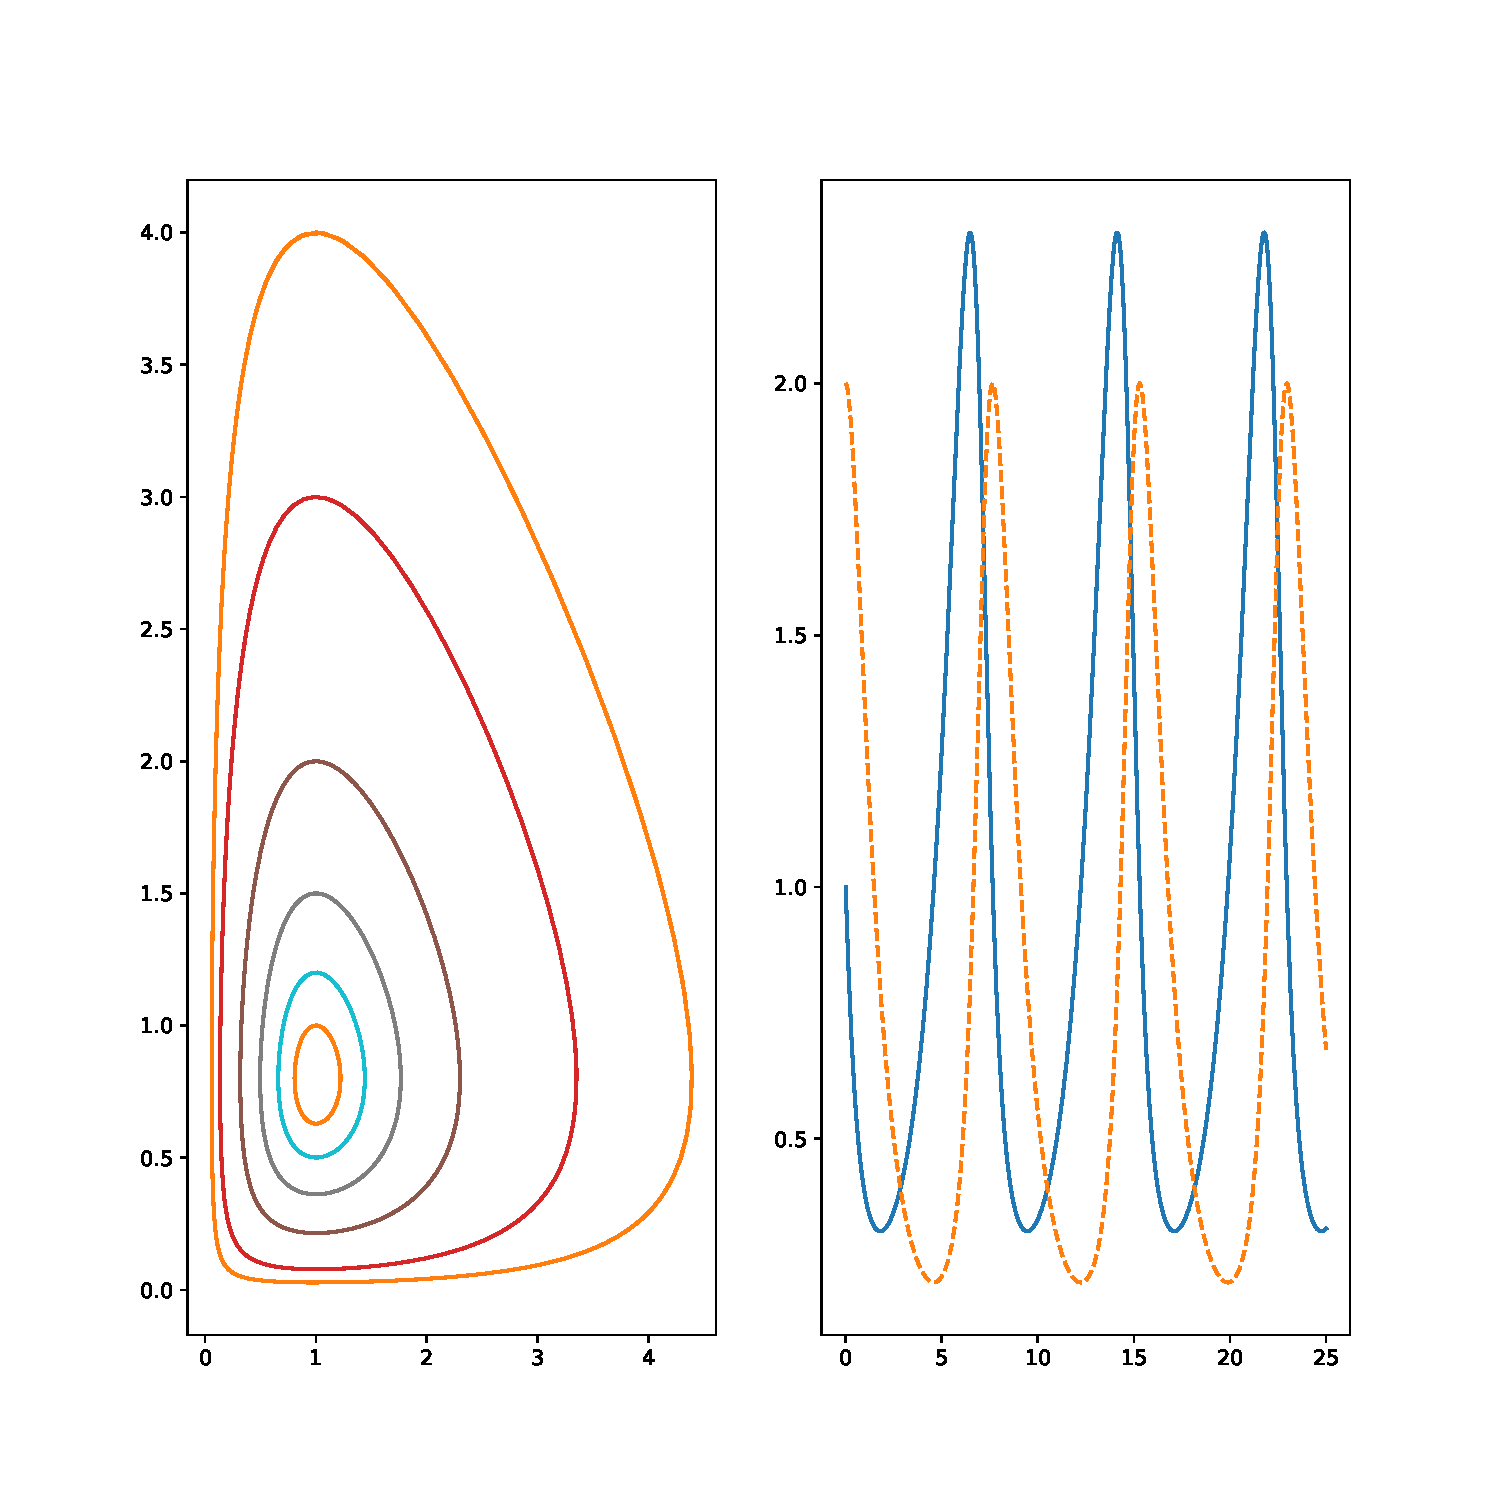
\includegraphics[scale = 0.6]{../figs/Lotka_Volterra.pdf} 
          \caption{Orbits of a Lotka Volterra system}
        \end{figure}

      \item
        The value of:
        \begin{equation*}
          L = f x + d \ln x - cy - a \ln y
        \end{equation*}

        \begin{figure}[H]
          \centering
          \includegraphics[scale = 0.6]{../figs/LVError.pdf}
          \caption{The value of $L$ along solutions}
        \end{figure}

      \item
        Numerical soution to a slightly perturbed problem.
        \begin{figure}[H]
          \centering
          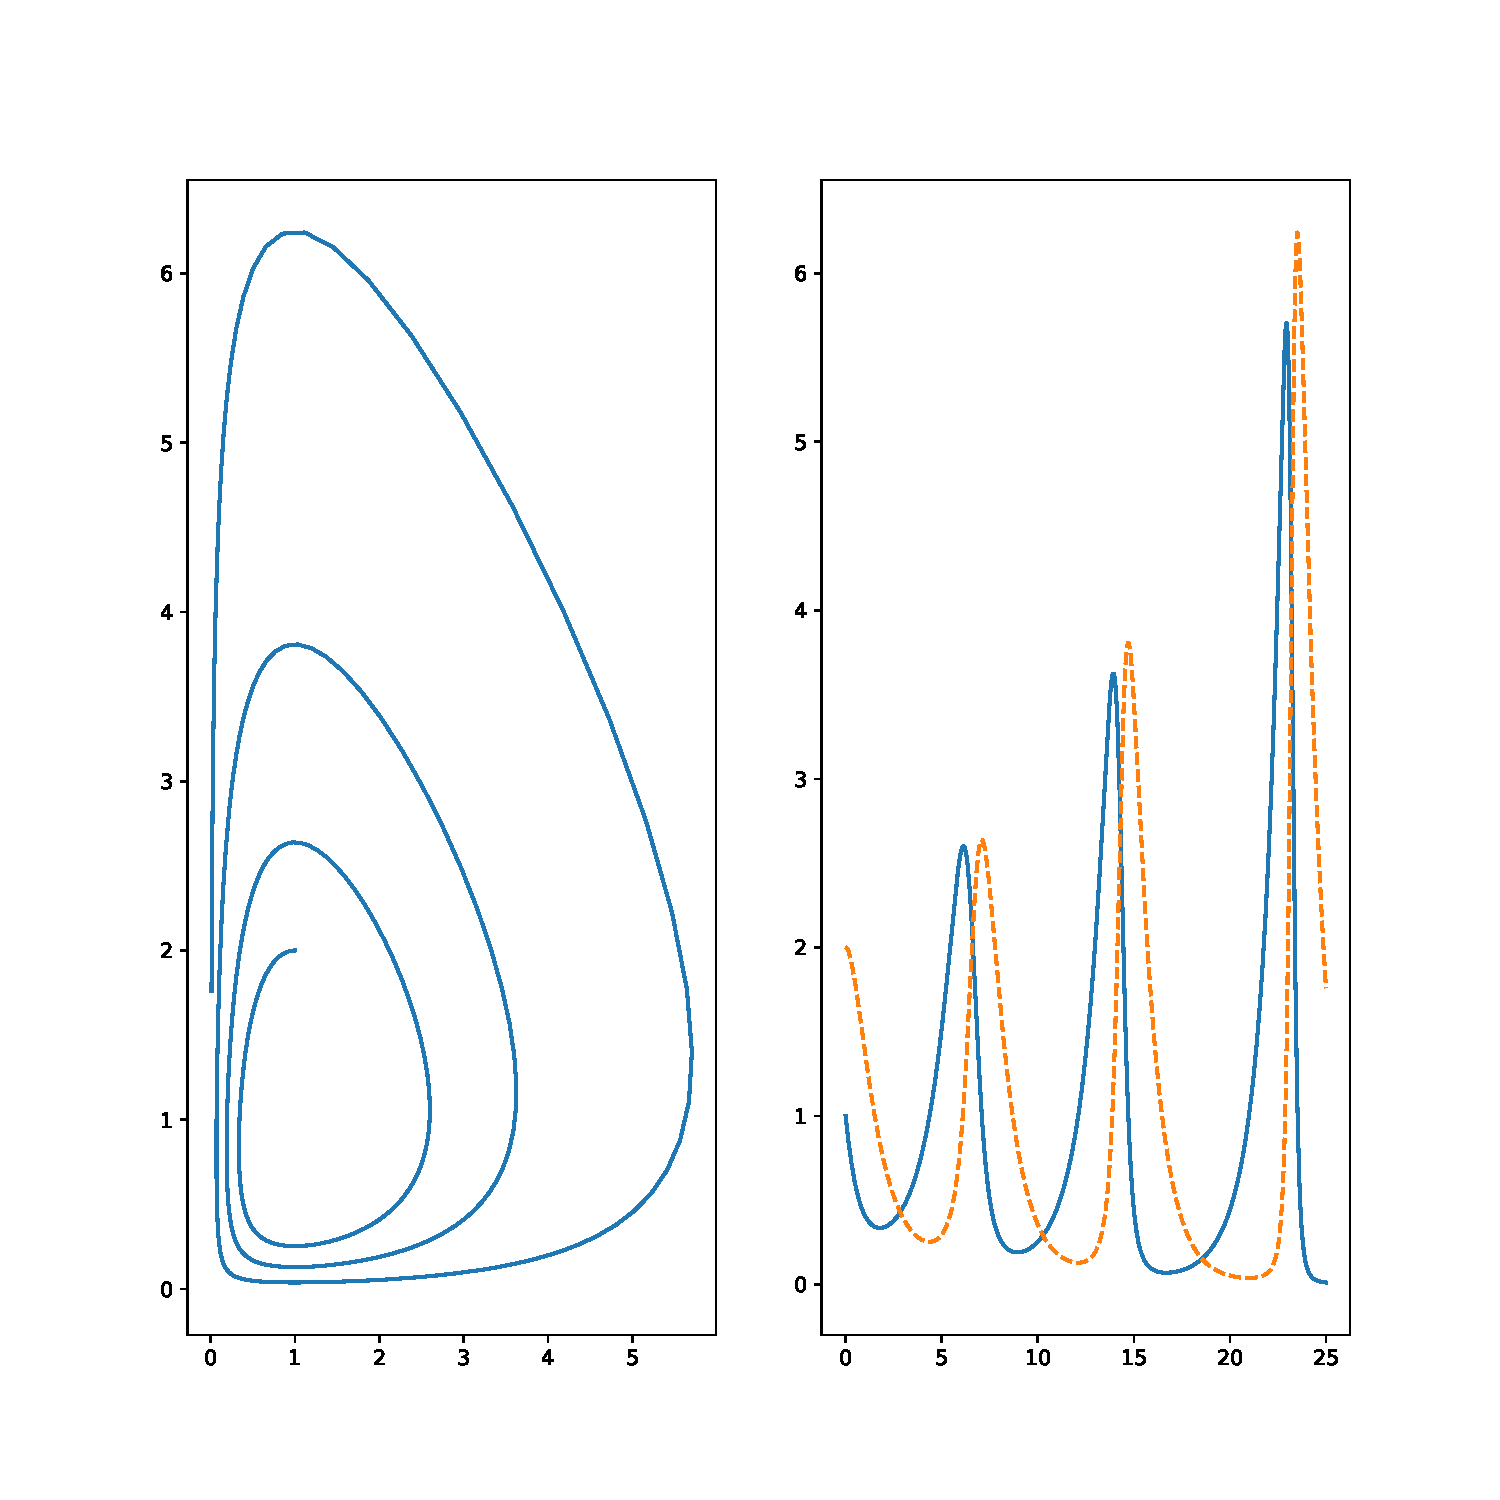
\includegraphics[scale = 0.6]{../figs/Lotka_Volterra0.1.pdf}
          \caption{Centered derivative and Euler Evolution of an advection equation  with $\Delta t = \Delta x$ and error}
        \end{figure}

    \end{enumerate}
  \item
    \begin{enumerate}
      \item
        SIR model.
        \begin{figure}[H]
          \centering
          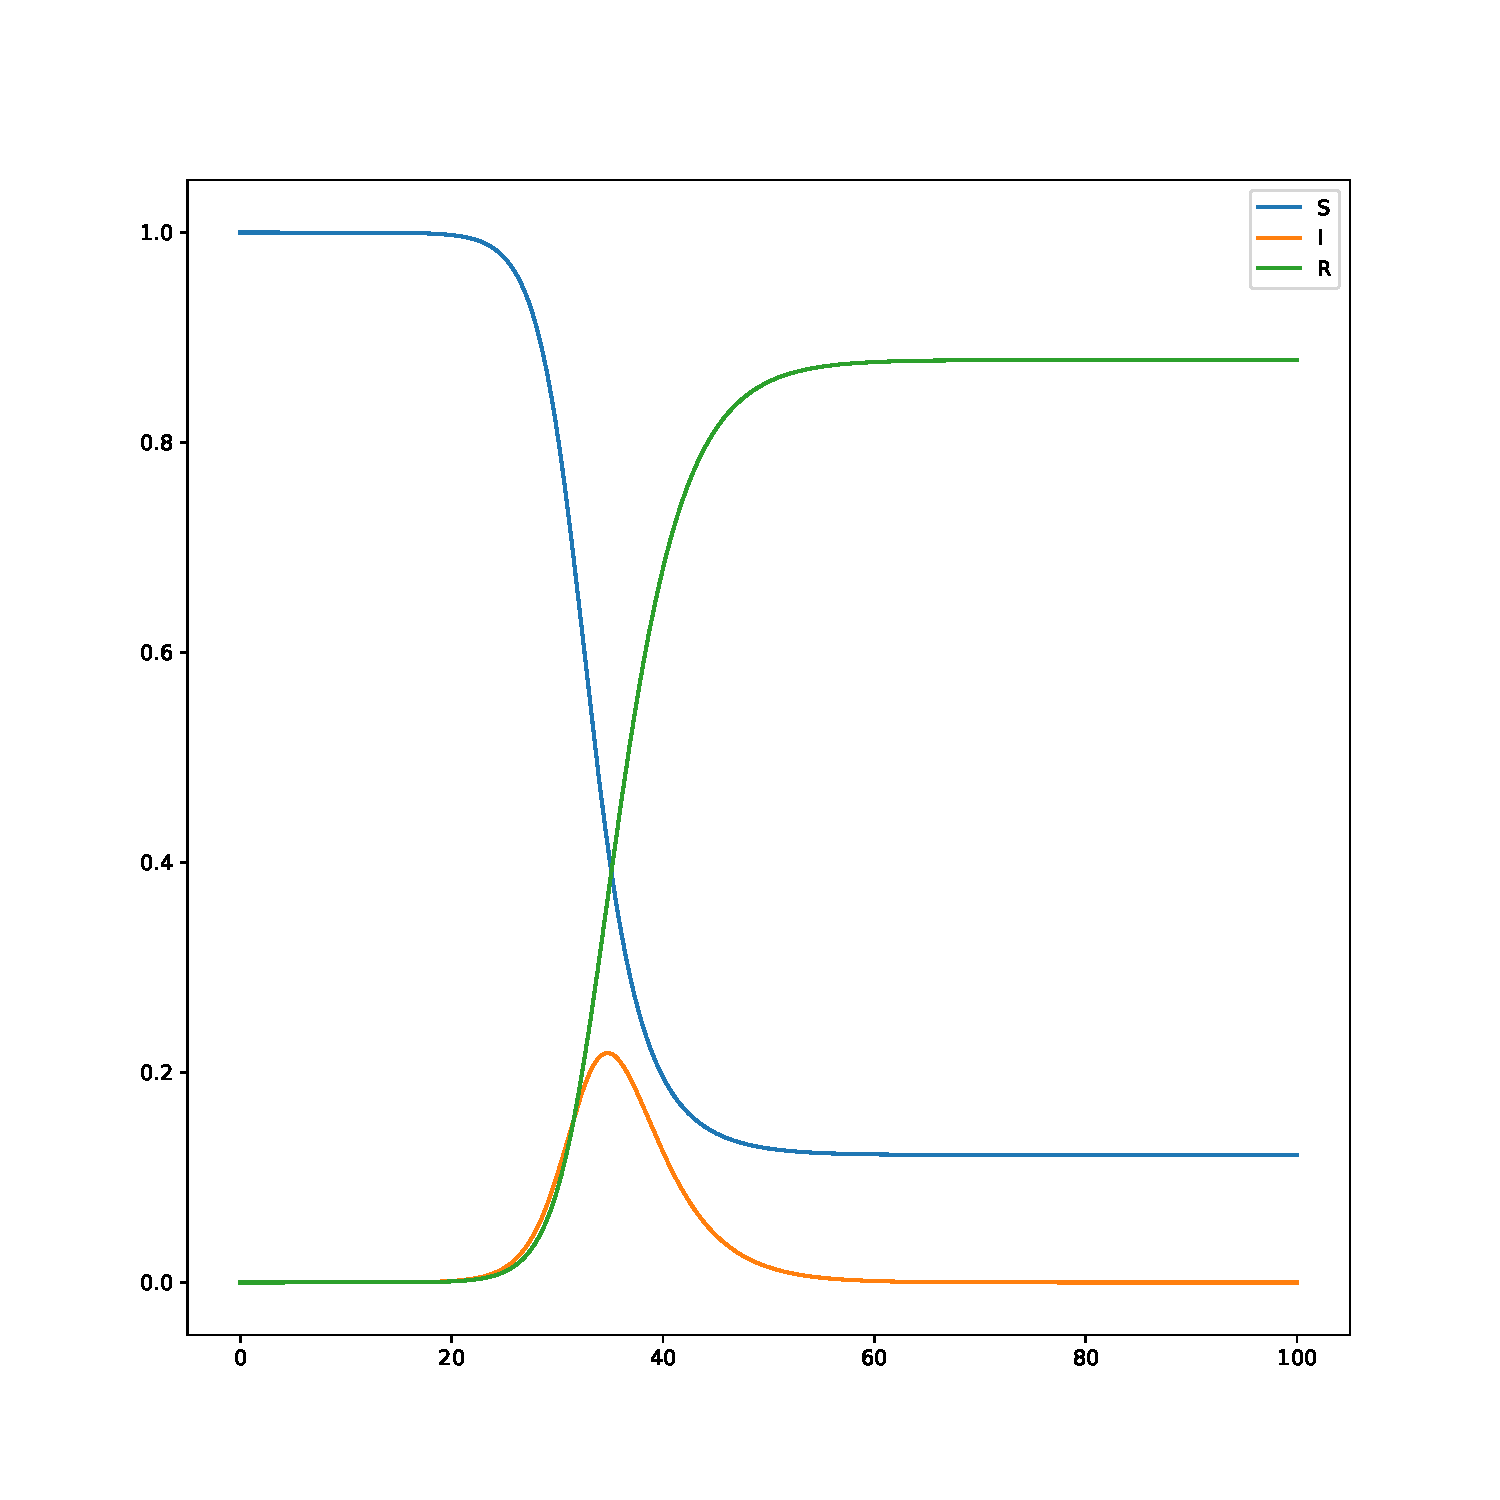
\includegraphics[scale = 0.9]{../figs/SIR.pdf}
          \caption{Evolution of an SIR model through time}
        \end{figure}

      \item
        Figure~\ref{fig:SIRbetaHalved} shows that halving $\beta$ (the contagiousness parameter) has a large impact on the infection curve.
        \begin{figure}[H]
          \centering
          \includegraphics[scale = 0.9]{../figs/SIRbetaHalved.pdf}
          \caption{Evolution of an SIR model through time}
          \label{fig:SIRbetaHalved}
        \end{figure}
  \end{enumerate}
  \item
    \begin{enumerate}
      \item
        Lorenz models are sensitive to initial conditions.
        Figure~\ref{fig:xvtLorenz} illustrates the chaos exihited by a Lorenz model.
        \begin{figure}[H]
          \centering
          \includegraphics[scale = 0.8]{../figs/xvtLorenz.pdf}
          \caption{Sensitivity of Lorenz system to initial conditions}
          \label{fig:xvtLorenz}
        \end{figure}
      \item
        Figure~\ref{fig:LorenzChaosTimeStep} illustrates the sensitivity solving of Lorenz model.
        The solution to the same problem results in substantially different solutions depending on the numerical integrator's time step.
        \begin{figure}[H]
          \centering
          \includegraphics[scale = 0.4]{../figs/LorenzChaosTimeStep.pdf}
          \caption{Chaos of Lorenz system when evolution time step is varied}
          \label{fig:LorenzChaosTimeStep}
        \end{figure}
      \item
        Figure~\ref{fig:lorenz} shows the lorenz model settling into two lobes.
        \begin{figure}[H]
          \centering
          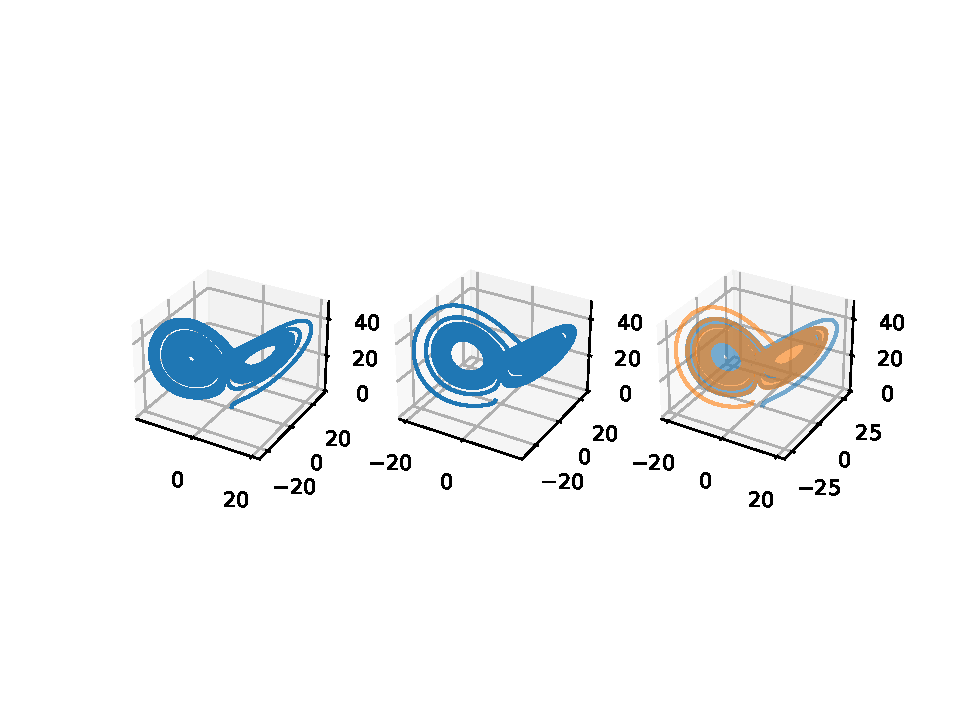
\includegraphics[scale = 0.7]{../figs/lorenz.pdf}
          \caption{3D plots of a Lorenz model}
          \label{fig:lorenz}
        \end{figure}
  \end{enumerate}
\end{enumerate}

\end{document}
